\documentclass[a4paper,11pt]{article}
\usepackage{geometry}
\usepackage[T1]{fontenc}
\usepackage[utf8]{inputenc}
\usepackage{lmodern}
\usepackage[francais]{babel}
\usepackage{authblk}
\usepackage{tabularx}
\usepackage{array}
\usepackage{listings}
\usepackage{color}
\usepackage{float}
\usepackage{graphicx}


\begin{document}

\begin{titlepage}
  \newcommand{\HRule}{\rule{\linewidth}{0.5mm}} % Defines a new command for the horizontal lines, change thickness here

  \center % Center everything on the page
   
  %----------------------------------------------------------------------------------------
  %	HEADING SECTIONS
  %----------------------------------------------------------------------------------------

  \textsc{\LARGE INSA de Lyon}\\[1.5cm] % Name of your university/college
  \textsc{\Large DASI}\\[0.5cm] % Major heading such as course name
  \textsc{\large Collect'IF : partie 1}\\[0.5cm] % Minor heading such as course title

  %----------------------------------------------------------------------------------------
  %	TITLE SECTION
  %----------------------------------------------------------------------------------------

  \HRule \\[0.4cm]
  { \huge \bfseries Dossier d'analyse}\\[0.1cm] % Title of your document
  \HRule \\[1.5cm]
   
  %----------------------------------------------------------------------------------------
  %	AUTHOR SECTION
  %----------------------------------------------------------------------------------------

  % If you don't want a supervisor, uncomment the two lines below and remove the section above
  \Large \emph{Auteurs:}\\[1cm]
  \newcolumntype{R}{>{\raggedleft\arraybackslash}X}
  \newcolumntype{L}{>{\raggedright\arraybackslash}X}
  \begin{table}[h]
    \begin{center}
      \begin{tabularx}{10cm}{R L}
         Pierre-louis & \textsc{Lefebvre} \\
         Nicolas & \textsc{Six} \\[5cm]
      \end{tabularx}
    \end{center}
  \end{table}
  
  %----------------------------------------------------------------------------------------
  %	DATE SECTION
  %----------------------------------------------------------------------------------------

  {\large \today}\\[3cm] % Date, change the \today to a set date if you want to be precise

  %----------------------------------------------------------------------------------------
  %	LOGO SECTION
  %----------------------------------------------------------------------------------------

  %\includegraphics{Logo}\\[1cm] % Include a department/university logo - this will require the graphicx package
   
  %----------------------------------------------------------------------------------------

  \vfill % Fill the rest of the page with whitespace

\end{titlepage}
\tableofcontents
\pagebreak

%end header

\section{Modèle du domaine}

\begin{figure}[h]
  \begin{center}
    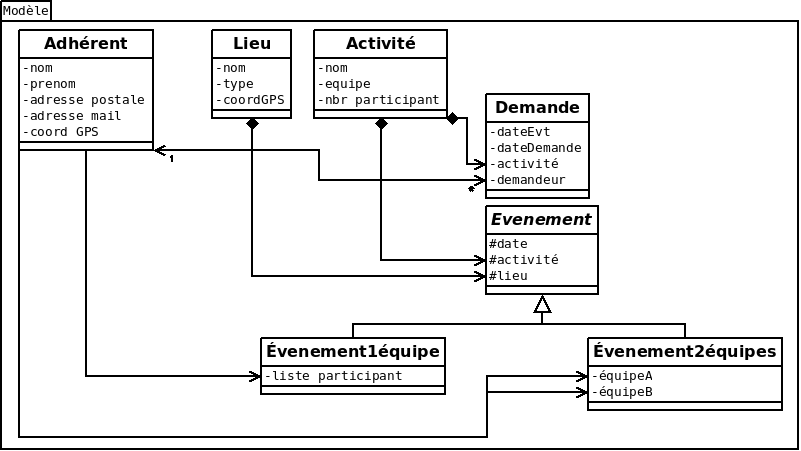
\includegraphics[width=10cm]{../modèle.png}
    \caption{Modèle du domaine}
  \end{center}
\end{figure}

\section{Maquette des IHMs}

\subsection{IHM utilisateur}

\subsubsection{Schema générale}

\begin{figure}[H]
  \begin{center}
    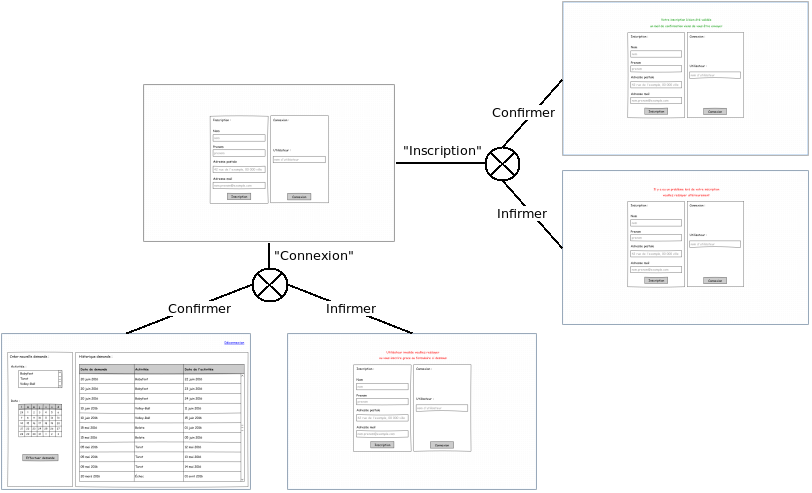
\includegraphics[width=14cm]{../../IHM/graphique_IHM.png}
    \caption{Modèle du domaine}
  \end{center}
\end{figure}

\subsubsection{IHM de connection du client}

\begin{figure}[H]
  \begin{center}
    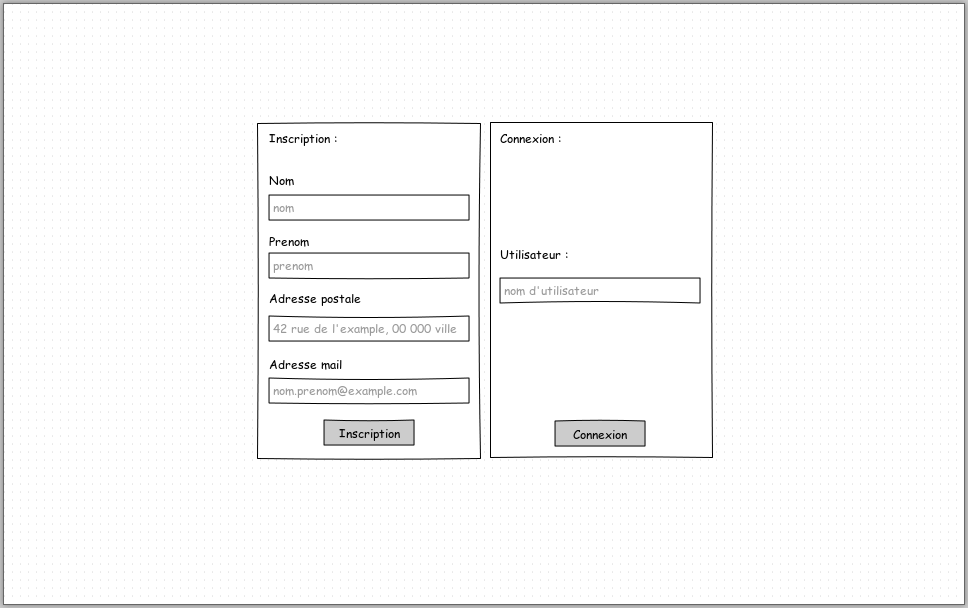
\includegraphics[width=12cm]{../../IHM/IHM connection utilisateur.png}
    \caption{Modèle du domaine}
  \end{center}
\end{figure}





\end{document}



